\section{Änderungen}
\begin{Change}{FeatureProvider}
    Die Funktionalität dieser Klasse sollte ursprünglich in 
    Controller.Frost.DataProvider enthalten sein und nach außen versteckt.
    Dies ermöglicht außerdem den 
    Zugriff auf die Features auch außerhalb des FROST-Pakets.
    
    \bigskip
    \textbf{Methoden}
    \begin{itemize}
        \item \texttt{static getInstance()}
        \\ Liefert die Singleton-Instanz zurück oder erstellt sie.
        \item \texttt{constructor()}
        \\ Initialisiert den Feature-Speicher und lädt die Definitionen
        \item \texttt{getFeature(id : string) : Feature|undefined}
        \\ Das gespeicherte Feature falls es existiert.
        Schlägt dies fehl wird 'undefined' zurückgegeben.
    \end{itemize}
\end{Change}

\begin{Change}{MapController}
    
    Skala und Viewport werden von außen lesbar gemacht.
    Damit muss MapPage keine eigene Kopie bereithalten.

    \bigskip
    \textbf{Hinzugefügt}
    \begin{itemize}
        \item \texttt{getScale() : Scale}
        \\ Die aktuelle Skala.
        \item \texttt{getViewport(): Viewport}
        \\ Der aktuelle Viewport.
    \end{itemize}

\end{Change}

\begin{Change}{OnSearch(string) für Suche}
    
    Die eigentliche Suche findet nun außerhalb der Komponente statt.
    Damit wird die Komponente leichter für verschiedene Anwendungen wiederverwendbar.

    \bigskip
    \textbf{Hinzugefügt}
    \begin{itemize}
        \item \texttt{Search.Props.onSearch(term: string) : void}
        \\ Wird bei Klick auf den Such-Button oder Drücken von Enter aufgerufen.
        Enthält den aktuellen Inhalt der Suchbox. 
        \item \texttt{MapView.onSearch(term: string) : void}
        \\ Ruft die Suche im MapController auf und aktualisiert die Seite.
    \end{itemize}

\end{Change}

\begin{Change}{Legend}
    
    Der Ausschnitt der von der Legende angezeigt wird soll flexibel sein.

    \bigskip
    \textbf{Hinzugefügt}
    \begin{itemize}
        \item \texttt{Props.min : number}
        \\ Das untere Ende der Legende
        \item \texttt{Props.max : number}
        \\ Das obere Ende der Legende
    \end{itemize}

\end{Change}

\begin{Change}{Map}
    
    Ursprünglich sollte der Viewport über die Mitte der Pins/Polygone bestimmt werden.
    Um die Karte von Anfang an auf die letzte Position zu zentrieren wird der Viewport direkt übergeben.
    
    \bigskip
    \textbf{Hinzugefügt}
    \begin{itemize}
        \item \texttt{Props.viewport : Viewport}
        \\ Viewport mit dem die Karte initialisiert wird.
    \end{itemize}

\end{Change}

\begin{Change}{FeatureSelectInit}
    
    Die FeatureSelect Auswahl benötigt die aktuellen Werte um sie standardmäßig auswählen zu können.
    
    \bigskip
    \textbf{Hinzugefügt}
    \begin{itemize}
        \item \texttt{FeatureSelect.Props.startConf?: \{ conf: string; feature: string \}}
        \\ Die Startwerte der Auswahlboxen. Optional.
        \item \texttt{MapController.getFeatureSelectConf(): { conf: string; feature: string }}
        \\ Gibt Werte für die Auswahlboxen basierend auf der Konfiguration aus.
    \end{itemize}

\end{Change}

\begin{Change}{Diagramme der Detailansicht}
    Im ursprünglichen Entwurf gab es eine abstrakte Diagrammklasse, die in unserer MVC-Architektur in der View zu verorten war. Unterschiedliche Diagramme sollten als unterschiedliche Klassen, die alle von der abstrakten Diagrammklasse erben, implementiert werden.
    Mit diesem Entwurf sind wir nun auf Probleme gestoßen, da React empfiehlt keine Vererbung von Komponenten zu verwenden, wodurch wir gezwungen waren unsere Modellierung zu verändern.

    Im Zuge dessen haben wir uns entschieden die Vererbung durch Komposition zu ersetzen. Nun gibt es weiterhin eine Diagrammklasse, die allerdings nun nicht abstrakt, sondern eine React Komponente ist, deren Aufgabe alleine im Anzeigen eines Diagramms besteht. Da wir zur Darstellung von Diagrammen "React Google Charts" verwenden dient die Diagrammklasse also nur als Adapter der Chart Komponente dieser Bibliothek.

    Die Differenzierung unterscheidlicher Diagrammtypen wird durch Komposition unterschiedlicher DiagramController erzielt, die einer Diagramm Komponente in den props übergeben werden. Ein DiagramController implementiert eine entsprechende Schnittstelle. Seine Aufgaben bestehen im Anfordern der diagrammspezifischen Daten vom DataProvider, dem Formatieren der Daten in ein zur Darstellung geeignetes Format und dem Wechsel zwischen unterschiedlicher Konfigurationsoptionen.

    Des Weiteren haben wir eine DiagramFactory Klasse mit einer statische Fabrikmethode ergänzt. Über diese ist es möglich mit einer typenId einen DiagrammController für ein bestimmtes Feature einer Messstation zu erzeugen. Diese Klasse hat im ursprünglichen Entwurf gefehlt, wodurch die Aufgabe im Model hätte erfolgen müssen, was allerding der MVC-Architektur widerspricht.

    Insgesamt harmoniert dieser neue Entwurf sehr viel besser mit React und unserer MVC-Architektur und vereinfacht zusätzlich den Code innerhalb der Diagrammklasse. Des Weiteren ist die Kopplung zwischen Inhalt und Darstellung eines Diagramms im neuen Entwurf sehr viel loser, wudurch es einfacher ist die Applikation durch neue Diagrammtypen zu ergänzen oder bestehende Diagrammtypen abzuändern.
    
    Das Klassendiagramm des neuen Entwurfs sieht nun wie folgt aus:
     \bigskip
    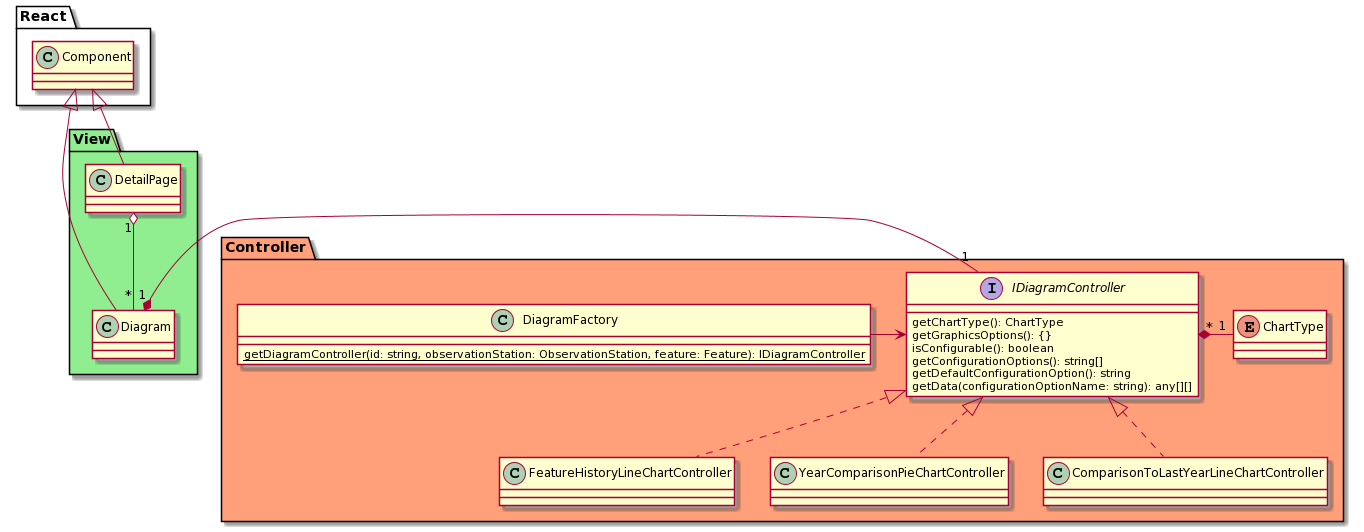
\includegraphics[width=1\linewidth]{Diagrams.png}\par\vspace{1cm}
    
\end{Change}

\begin{Change}{IDs für MapConfiguration}
    Ursprünglich sollte die Art der Konfiguration über das name Attribut bestimmt werden.
    Das führt aber im build zu Problemen da Klassennamen komprimiert werden.

    \textbf{Hinzufügen}
    \begin{itemize}
        \item \texttt{abstract getId() : string}
        \\ Die ID der Karten-Konfiguration
    \end{itemize}
\end{Change}

\begin{Change}{Featurespezifische Icons}
    Jedes Feature besitzt nun eine eigenes Icon. Das Icon wird über den Konstruktor übergeben.

    \textbf{Hinzufügen}
    \begin{itemize} 
        \item \texttt{abstract getId() : string}
        \\ Die ID der Karten-Konfiguration
    \end{itemize}
    
\end{Change}

\begin{Change}{ObservationItem}
    Um den Code in der Klasse ObservationStationProfile zu vereinfachen haben wir eine Klasse ObservationItem ergänzt. Ein ObservationItem ist ein Punkt in der Liste der letzten gemessenen Werte. Als reine View Komponente zeigt ein ObservationItem also einen Messwert, das jeweilige Feature und ein featurespezifisches Icon an.
\end{Change}

\begin{Change}{App Configuration}
    Es wurde eine eigene Klasse für die Anwendungskonfiguration erstellt (Singleton)
    um eventuelle neue Einstellungen möglichst einfach hinzufügen zu können.
    In einer config.json befindet sich ein Objekt des Typs IConfig
    \textbf{Hinzugefügt}
    \begin{itemize}
        \item \texttt{Configuration.getInstance()}
        \\ Lädt die Konfigurationsdatei in das Singleton-Objekt
        \item \texttt{Configuration.getLanguage()}
        \\ Die Standard 
        \item \texttt{Configuration.getFrostUrl()}
        \\ Das Top-Level der FROST-REST-API
        \item \texttt{interface IConfig}
        \\ frostUrl: string;
        \\ language: string;
        \\ supportedFeatures: string[];
    \end{itemize}
\end{Change}

\begin{Change}{IDs für MapConfiguration}
    Um die verschiedenen Konfigurationen ohne fehleranfällige typeof Abfragen unterscheiden
    zu können wurden IDs hinzugefügt die i.d.R. als Konstante gespeichert sind.
    \begin{itemize}
        \item \textbf{MapConfiguration.getID() : string}
        \\ Eine eindeutige Kennung der MapConfiguration nach Typ.
    \end{itemize}
\end{Change}

\begin{Change}{ObservationItem}
    Um den Code in der Klasse ObservationStationProfile zu vereinfachen haben wir eine Klasse ObservationItem ergänzt. Ein ObservationItem ist ein Punkt in der Liste der letzten gemessenen Werte. Als reine View Komponente zeigt ein ObservationItem also einen Messwert, das jeweilige Feature und ein featurespezifisches Icon an.
\end{Change}
